\documentclass{article}
\usepackage{amsmath}
\usepackage{tikz}
\usepackage{mathtools}
\usepackage[a4paper, total={6in, 8in}]{geometry}
\usepackage{amssymb}
\usepackage{color}
\usepackage{lscape}
\usepackage{listings}
\usepackage{xcolor}
\usepackage{float}
\usepackage{hyperref}
\usepackage{fancyhdr}
\pagestyle{fancy}

% Define the header
\fancyfoot[R]{Fernando Urbano}
\renewcommand{\footrulewidth}{0.2pt}

\fancyhead[L]{ECMA 31380 - Causal Machine Learning}
\fancyhead[R]{Proposal Final Project}

\usepackage{graphicx}
\setlength{\parskip}{0.5em}
\setlength{\parindent}{0pt}
\renewcommand{\thesubsection}{\thesection.\arabic{subsection}}
\newcommand{\divider}{\vspace{1em}\hrule\vspace{1em}}

\definecolor{codegreen}{rgb}{0,0.6,0}
\definecolor{codegray}{rgb}{0.5,0.5,0.5}
\definecolor{codepurple}{rgb}{0.58,0,0.82}
\definecolor{backcolour}{rgb}{0.95,0.95,0.92}

\lstdefinestyle{Rstyle}{
  backgroundcolor=\color{backcolour},   
  commentstyle=\color{codegreen},
  keywordstyle=\color{blue},
  numberstyle=\tiny\color{codegray},
  stringstyle=\color{codepurple},
  basicstyle=\ttfamily\footnotesize,
  breakatwhitespace=false,         
  breaklines=true,                 
  captionpos=b,                    
  keepspaces=true,                 
  numbers=left,                    
  numbersep=5pt,                  
  showspaces=false,                
  showstringspaces=false,
  showtabs=true,                  
  tabsize=2,
  language=R
}

\title{ECMA 31380 - Proposal Final Project}
\author{Fernando Rocha Urbano}
\date{Autumn 2024}

% Define colors
\definecolor{codegreen}{rgb}{0,0.6,0}
\definecolor{codegray}{rgb}{0.5,0.5,0.5}
\definecolor{codepurple}{rgb}{0.58,0,0.82}
\definecolor{backcolour}{rgb}{0.95,0.95,0.92}

% Setup the listings package
\lstdefinestyle{Python}{
    backgroundcolor=\color{backcolour},   
    commentstyle=\color{codegreen},
    keywordstyle=\color{magenta},
    numberstyle=\tiny\color{codegray},
    stringstyle=\color{codepurple},
    basicstyle=\ttfamily\footnotesize,
    breakatwhitespace=false,         
    breaklines=true,                 
    captionpos=b,                    
    keepspaces=true,                 
    numbers=left,                    
    numbersep=5pt,                  
    showspaces=false,                
    showstringspaces=false,
    showtabs=false,                  
    tabsize=2
}

\newenvironment{colorparagraph}[1]{\par\color{#1}}{\par}
\definecolor{questioncolor}{RGB}{20, 40, 150}
\definecolor{tacolor}{RGB}{200, 0, 0}
% \documentclass[tikz,border=2mm]{standalone}
% \lstset{style=mystyle}
\usetikzlibrary{arrows.meta, positioning}


\begin{document}

\maketitle

\section{Goal}

The goal of this project is to evaluate the performance of different Double Machine Learning (DML) models in recovering the Average Treatment Effect (ATE) across various causal inference scenarios addressed in simulations.

The desired broader impact of the project is to provide actionable recommendations for selecting the most appropriate DML method based on the causal scenario, data structure, noise levels, and sample size. Additionally, we aim to create a benchmarking framework that practitioners can use to evaluate and compare causal inference estimates derived from the tested methods in different scenarios.

The DML methods compared in this study are:
\begin{itemize}
    \item LASSO.
    \item Random Forest.
    \item Neural Networks.
\end{itemize}

The causal inference scenarios are:
\begin{itemize}
    \item Backdoor adjustment.
    \item Frontdoor adjustment with and without access to mediators.
    \item Instrumental Variables with varying levels of instrument strength and correct vs. incorrect use of the IV.
\end{itemize}

We explore how each model implementation performs under varying conditions:
\begin{itemize}
    \item Relationships as linear and non-linear between covariates and treatment and between covariates and target $(g(\cdot) \ \text{and} \ m(\cdot))$.
    \item Noise levels $(\varepsilon)$.
    \item Sample size $(n)$.
    \item Size of high-dimensional impactful covariates $(d_c)$.
    \item Size of high-dimensional irrelevant covariates $(d_a)$.
\end{itemize}

For each of the scenario combinations, we show which of LASSO, Random Forest and Neural Networks provides more accurate ATE estimates based on the following metrics.
\begin{itemize}
    \item Bias of $\hat{\text{ATE}}$.
    \item Variance of $\hat{\text{ATE}}$ across repeated simulations for a given scenario.
    \item Analytical Variance of the $\hat{\text{ATE}}$.
    \item MSE (Mean Squared Error).
\end{itemize}

\section{Methodology}

\subsection{Problem Setup}

Consider a random sample ${(Y_i, T_i, X_i)}_{i=1}^n$, where:
\begin{itemize}
\item $Y_i \in \mathbb{R}$ is the outcome variable.
\item $T_i \in {0,1}$ is a binary treatment indicator.
\item $X_i \in \mathbb{R}^p$ is a vector of covariates.
\end{itemize}

Our goal is to estimate the Average Treatment Effect (ATE), defined as:
\begin{equation}
\tau = \mathbb{E}[Y_i(1) - Y_i(0)],
\label{eq:tau_hat_potential_outcome}
\end{equation}
where $Y_i(t)$ denotes the potential outcome for unit $i$ under treatment $T_i = t$.

\subsection{Identification via Conditional Expectations}

Under the Conditional Independence Assumption (CIA) and overlap conditions, the ATE can be identified as:
\begin{equation}
\tau = \mathbb{E}[\mu_1(X_i) - \mu_0(X_i)],
\label{eq:tau_hat_potential_outcome_diff_means}
\end{equation}
where $\mu_t(X_i) = \mathbb{E}[Y_i | T_i = t, X_i]$ is the conditional expectation of the outcome given treatment and covariates.

\subsection{Double Machine Learning (DML) Estimator}

The DML framework aims to estimate $\tau$ while controlling for high-dimensional or complex relationships between $Y_i$, $T_i$, and $X_i$. The key idea is to use machine learning methods to estimate the nuisance parameters and then construct an estimator for $\tau$ that is robust to estimation errors in these nuisance parameters.

\subsubsection{Nuisance Parameter Estimation}

We define the following nuisance functions:
\begin{align}
& m(X_i) = \mathbb{E}[Y_i | X_i],
\label{eq:m_x_for_target}
\\
& g(X_i) = \mathbb{E}[T_i | X_i],
\label{eq:g_x_for_treatment}
\\
& \pi(X_i) = \mathbb{P}(T_i = 1 | X_i) \quad \text{(propensity score)}
\label{eq:pi_x_for_treatment}
\end{align}

These functions can be estimated using flexible machine learning methods such as LASSO, Random Forests, or Neural Networks.

Under mild regularity conditions and appropriate rates of convergence for the nuisance estimators, the DML estimator is root-n consistent and asymptotically normal. It provides valid confidence intervals and hypothesis tests even when using complex machine learning methods for $\hat{m}(X)$ and $\hat{g}(X)$.

\subsubsection{Orthogonal Score Function}

To achieve robustness, we construct an orthogonal score function $\psi(Y_i, T_i, X_i; \eta)$, where $\eta = (m, g)$ represents the nuisance parameters. The orthogonal score satisfies the Neyman orthogonality condition, which ensures that small estimation errors in $\eta$ have a negligible first-order impact on the estimation of $\tau$.

A common choice for the orthogonal score is:
\begin{equation}
\psi(Y_i, T_i, X_i; \eta) = \left( \frac{T_i - g(X_i)}{\pi(X_i)(1 - \pi(X_i))} \right) (Y_i - m(X_i)) + \left( m_1(X_i) - m_0(X_i) \right) - \tau,
\label{eq:orthogonal_score}
\end{equation}

where $g(X_i) = \pi(X_i)$ in case of binary treatment and:

\begin{equation}
m_t(X_i) = \mathbb{E}[Y_i | T_i = t, X_i]  \quad \text{for} \ t \in \{0,1\}
\label{eq:orthogonal_score_m_t}
\end{equation}

\subsubsection{Estimation Procedure}

The estimation proceeds in several steps:
\begin{enumerate}
\item Estimate Nuisance Functions: Use one of the three outline ML models to obtain estimators $\hat{m}(X_i)$ and $\hat{g}(X_i)$ for the nuisance functions.

\item Compute the Score Function: Evaluate the orthogonal score $\psi(Y_i, T_i, X_i; \hat{\eta})$ using the estimated nuisance parameters.

\item Estimate $\tau$: Solve the empirical moment condition which yields $\hat{\tau}$:

\begin{equation}
\frac{1}{n} \sum_{i=1}^n \psi(Y_i, T_i, X_i; \hat{\eta}) = 0.
\label{eq:orthogonal_score_psi}
\end{equation}
\end{enumerate}

The orthogonal score function mitigates the impact of errors in $\hat{m}(X)$ and $\hat{g}(X)$ on the estimation of $\tau$ while also accomodating the use of modern ML techniques, allowing complex relationships between $Y$, $X$ and $T$.

To prevent overfitting and ensure that the estimation error in the nuisance parameters does not bias the estimator of $\tau$ we employ cross-fitting.

\subsubsection{Cross-Fitting}

The steps of cross-fitting are:

\begin{enumerate}
\item Split the Sample: Divide the data into K folds $\{\mathcal{I}_k\}{k=1}^K$.
\item For Each Fold:
\begin{enumerate}
\item Train Nuisance Estimators: Use data from all other folds:
$$
\mathcal{I}_{-k} = \bigcup{j \neq k} \mathcal{I}_j
$$
to estimate $\hat{m}^{(-k)}(X_i)$ and $\hat{g}^{(-k)}(X_i)$.

\item Compute Score Function: For observations in fold $\mathcal{I}_k$, compute $\psi(Y_i, T_i, X_i; \hat{\eta}^{(-k)})$ using the nuisance estimates from step (a):

\begin{equation}
    \begin{split}
        \psi(Y_i, T_i, X_i; \hat{\eta}^{(-k)}) = & \left( \frac{T_i - \hat{g}^{(-k)}(X_i)}{\hat{\pi}^{(-k)}(X_i)} \right) (Y_i - \hat{m}^{(-k)}(X_i)) \\
        & + \ \hat{m}_1^{(-k)}(X_i) - \hat{m}_0^{(-k)}(X_i) - \tau^{(-k)}.
    \end{split}
    \label{eq:orthogonal_score_fold_k}
\end{equation}

\end{enumerate}
\item Aggregate: Combine the estimates from all folds:

\begin{equation}
\hat{\tau} = \frac{1}{n} \sum_{k=1}^K \sum_{i \in \mathcal{I}_k} \hat{\tau}_i^{(-k)} =  \frac{1}{K} \sum_{k=1}^K \hat{\tau}^{(-k)}
\label{eq:avg_tau_hat}
\end{equation}

\end{enumerate}

\section{Causal Inference Scenarios}

The three most relevant scenarios of causal inference are the ones that require Instrumental Variables, Backdoor Adjustment, or Front Door Adjustment. A common way to represent the causal relation related to those is through the use of DAGs.

\subsection{DAG (Directed Acyclic Graph)}

Directed Acyclic Graph (DAG) serves as a representation of causal assumptions and a tool for deriving statistical properties of the variables involved.

It is composed of nodes (vertices) representing random variables or features and directed edges (arrows), indicating a direct influence or causal effect of $T$ on $Y$.

\begin{figure}[H]
    \centering
    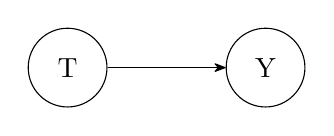
\begin{tikzpicture}[
        >={Stealth[round]},
        every node/.style={draw, circle, minimum size=1cm},
        every edge/.style={draw, ->, thick},
        node distance=2cm
    ]
    
    \node (T) {T};
    \node (Y) [right=of T, xshift=-0.5cm] {Y};
    
    \draw[->] (T) -- (Y);
    \end{tikzpicture}
    \label{fig:dag_example}
    \caption{DAG Example}
\end{figure}

The acyclic characterist is due to absence of directed cycles; that is, there is no path where you can start at a node $X$ and, by following directed edges, return to $X$.

\subsection{Backdoor Adjustment}

A backdoor path from treatment $T$ to the outcome $Y$ represents alternative routes through which association can flow from $T$ to $Y$ that are not due to the causal effect of $T$ on $Y$. In the representation, the confounder $C$ is a common cause of both $T$ and $Y$, thus, a backdoor path.

In such case, the association between $T$ and $Y$ may be partially or entirely due to their mutual dependence on $C$ rather than a direct causal effect, leading to biased causal estimates of the treatment if $C$ is ignored.

The causal effect of $T$ on $Y$ can be expressed using the backdoor adjustment formula:

\begin{equation}
    \mathbb{P}[Y(t)] = \sum_C \mathbb{P}[Y \mid T, C] \mathbb{P}[C],
\end{equation}

Which serves a markov factorization, calculating with respect to the DAG structure.

For the backdoor adjustment to be valid, the following conditions must be satisfied:

\begin{enumerate}
    \item No variable in the adjustment set is a descendant of the treatment $T$.
    \item The adjustment set blocks all backdoor paths from $T$ to $Y$ (backdoor path is any path from $T$ to $Y$ that starts with an arrow into $T$).
\end{enumerate}

DAG~\ref{fig:dag_backdoor_path} illustrates the backdoor path involving the confounder $C$, treatment $T$, outcome $Y$, and features with non-causal association $X_a$ which would not be present in a typical backdoor adjustment DAG, but play a relevant role in the simulations proposed.

\begin{figure}[H]
    \centering
    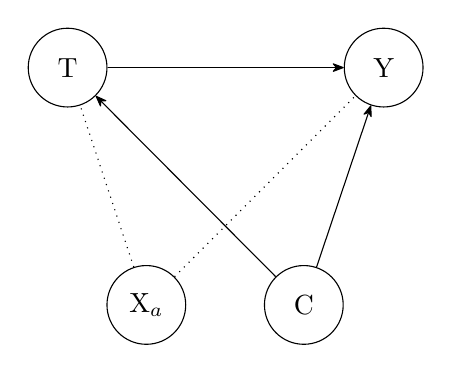
\begin{tikzpicture}[
        >={Stealth[round]},
        every node/.style={draw, circle, minimum size=1cm},
        every edge/.style={draw, ->, thick},
        node distance=2cm
    ]
    
    \node (T) {T};
    % \node (C) [above=of T, xshift=1.5cm] {C};
    \node (Y) [right=of T, xshift=1cm] {Y};
    \node (XC) [below=of T, xshift=3cm] {$\text{C}$};
    \node (XA) [below=of T, xshift=1cm] {$\text{X}_a$};
    
    % \draw[->] (C) -- (T);
    % \draw[->] (C) -- (Y);
    \draw[->] (T) -- (Y);  
    \draw[->] (XC) -- (T);
    \draw[->] (XC) -- (Y);
    \draw[dotted] (XA) -- (T);
    \draw[dotted] (XA) -- (Y);
    \end{tikzpicture}
    \label{fig:dag_backdoor_path}
    \caption{DAG of Backdoor Path}
\end{figure}

\subsection{Frontdoor Adjustment}

Frontdoor adjustment is a method used to estimate the causal effect of treatment $T$ on outcome $Y$ when there is unmeasured confounding that cannot be addressed using backdoor adjustment. It leverages a mediator $M$ that lies on the causal path from $T$ to $Y$.

The causal effect of $T$ on $Y$ can be expressed using the frontdoor adjustment formula:

\begin{equation}
\mathbb{P}[Y(t)] = \sum_M \mathbb{P}[M \mid T=t] \sum_{t’} \mathbb{P}[Y \mid M, T=t’] \mathbb{P}[T=t’].
\end{equation}

For the frontdoor adjustment to be valid, the following conditions must be satisfied:

\begin{enumerate}
\item All causal paths from $T$ to $Y$ pass through $M$ (i.e., there is no direct effect of $T$ on $Y$ bypassing $M$).
\item There are no unmeasured confounders between $T$ and $M$.
\item All backdoor paths from $M$ to $Y$ are blocked by $T$ (i.e., there are no unmeasured confounders between $M$ and $Y$ that are not affected by $T$).
\end{enumerate}

DAG~\ref{fig:dag_frontdoor_path} illustrates the frontdoor adjustment involving the confounder $C$, treatment $T$, mediator $M$, outcome $Y$, and features with non-causal association $X_a$, which are included due to their relevance in the proposed simulations.

\begin{figure}[H]
    \centering
    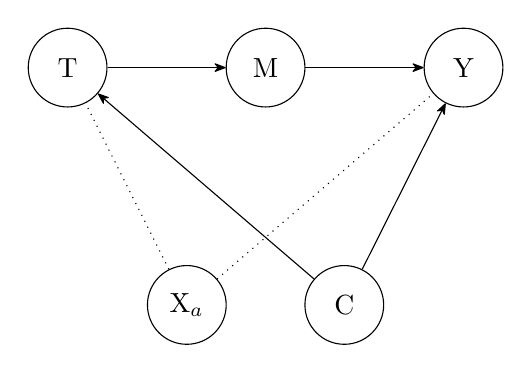
\begin{tikzpicture}[
        >={Stealth[round]},
        every node/.style={draw, circle, minimum size=1cm},
        every edge/.style={draw, ->, thick},
        node distance=2cm
    ]
    
    \node (T) {T};
    \node (M) [right=of T, xshift=-0.5cm] {M};
    \node (Y) [right=of M, xshift=-0.5cm] {Y};
    \node (XA) [below=of M, xshift=-1cm] {$\text{X}_a$};
    \node (XC) [below=of M, xshift=1cm] {C};
    
    \draw[->] (T) -- (M);
    \draw[->] (M) -- (Y);
    \draw[->] (XC) -- (T);
    \draw[->] (XC) -- (Y);
    \draw[dotted] (XA) -- (T);
    \draw[dotted] (XA) -- (Y);
    \end{tikzpicture}
    \label{fig:dag_frontdoor_path}
    \caption{DAG of Frontdoor Path}
\end{figure}

\subsection{Instrumental Variable}

Instrumental variable (IV) estimation is a method used to estimate the causal effect of a treatment  T  on an outcome  Y  when there is unmeasured confounding that cannot be addressed using backdoor or frontdoor adjustments. This method leverages an instrument  Z , which influences the treatment  T  but has no direct effect on the outcome  Y  except through  T , and is independent of any unmeasured confounders  U  affecting both  T  and  Y .

The causal effect of  T  on  Y  can be estimated using the instrumental variable formula:

\begin{equation}
\text{Causal Effect} = \frac{\text{Cov}(Z, Y)}{\text{Cov}(Z, T)}.
\end{equation}

Alternatively, in terms of expectations for a binary instrument  Z :

\begin{equation}
\text{Causal Effect} = \frac{\mathbb{E}[Y \mid Z = 1] - \mathbb{E}[Y \mid Z = 0]}{\mathbb{E}[T \mid Z = 1] - \mathbb{E}[T \mid Z = 0]}.
\end{equation}

For the instrumental variable method to be valid, the following conditions must be satisfied:

\begin{enumerate}
\item Relevance: The instrument $Z$ is associated with the treatment  $T$  (i.e.,  $\text{Cov}(Z, T) \neq 0$  or \( Z \not\!\perp\!\!\!\perp T \)).
\item Exclusion Restriction: The instrument $Z$ affects the outcome $Y$ only through its effect on the treatment $T$ (i.e., there is no direct effect of $Z$ on $Y$ and no other pathways from $Z$ to $Y$ except through  $T$).
\item Independence (Ignorability): The instrument $Z$ is independent of any unmeasured confounders $U$ that affect both $T$ and $Y$ $(i.e.,  Z \perp\!\!\!\perp U )$.
\end{enumerate}

DAG~\ref{fig:dag_instrumental_variable} illustrates the instrumental variable setup involving the unobserved confounder $U$, instrument $Z$, treatment $T$, outcome $Y$, observed confounder $C$, and features with non-causal associations $X_a$, which are included due to their relevance in the proposed simulations.

\begin{figure}[H]
    \centering
    \begin{tikzpicture}[
        >={Stealth[round]},
        every node/.style={draw, circle, minimum size=1cm},
        every edge/.style={draw, ->, thick},
        node distance=2cm
    ]
    
    \node (Z) {Z};
    \node (T) [right=of Z] {T};
    \node (U) [above=of T, xshift=2cm, yshift=-1cm, dashed] {U};
    \node (XC) [below=of T, xshift=1cm] {$\text{C}$};
    \node (XA) [below=of T, xshift=3cm] {$\text{X}_a$};
    \node (Y) [right=of T, xshift=1cm] {Y};
    
    \draw[->] (Z) -- (T);
    \draw[->] (T) -- (Y);
    \draw[->] (U) -- (T);
    \draw[->] (U) -- (Y);
    \draw[->] (XC) -- (T);
    \draw[->] (XC) -- (Y);
    \draw[dotted] (XA) -- (T);
    \draw[dotted] (XA) -- (Y);
    \end{tikzpicture}
    \label{fig:dag_instrumental_variable}
    \caption{DAG of Instrumental Variable}
\end{figure}

\end{document}
